
%(BEGIN_QUESTION)
% Copyright 2010, Tony R. Kuphaldt, released under the Creative Commons Attribution License (v 1.0)
% This means you may do almost anything with this work of mine, so long as you give me proper credit

Sketch the necessary wire connections so that the proximity switch sends a signal to channel {\tt IN3} on the correct discrete input card:

$$\includegraphics[width=15.5cm]{i02178x01.eps}$$

Note that the proximity switch is of the {\it sinking} type (NPN, or ``low-side''), and the PLC has two discrete input cards: one {\it sourcing} and one {\it sinking}.  The power supply module on the left-hand side of the PLC rack provides two screw terminals for 24 volt DC power to run the proximity switch.

\underbar{file i02178}
%(END_QUESTION)





%(BEGIN_ANSWER)

$$\includegraphics[width=15.5cm]{i02178x02.eps}$$

%(END_ANSWER)





%(BEGIN_NOTES)

{\bf This question is intended for exams only and not worksheets!}.

%(END_NOTES)

